% !TEX root = ../main.tex
%---------------------------------------------------------------------------------------------------
%---------------------------------------------------------------------------------------------------
\section{Empirical setup}\addtocounter{framenumber}{-1}
%---------------------------------------------------------------------------------------------------
%---------------------------------------------------------------------------------------------------
\begin{frame}\frametitle{Eckstein--Keane--Wolpin models}

\begin{multicols}{2}

	\heading{Understanding individual decisions}\vspace{0.3cm}
	\begin{itemize}\setlength\itemsep{1em}
		\item Human capital investment
		\item Consumption--savings decision
	\end{itemize}

    \pause

	\heading{Predicting effects of policies}\vspace{0.3cm}
	\begin{itemize}\setlength\itemsep{1em}
		\item Educational policy
		\item Welfare programs
	\end{itemize}

\end{multicols}

\pause
\heading{Mathematical framework and implementation}\vspace{0.3cm}
\begin{itemize}\setlength\itemsep{1em}
 \item Finite-horizon discrete Markov decision problem
 \item Backward induction algorithm
\end{itemize}

\end{frame}
%---------------------------------------------------------------------------------------------------
%---------------------------------------------------------------------------------------------------
\begin{frame}{Timing of events}
\vspace{0.5cm}
\scalebox{0.9}{\hspace{-0.2cm}%!TEX root = ../main.tex
% \definecolor{gray}{RGB}{31,119,180}

% \definecolor{light-gray}{gray}{0.85}


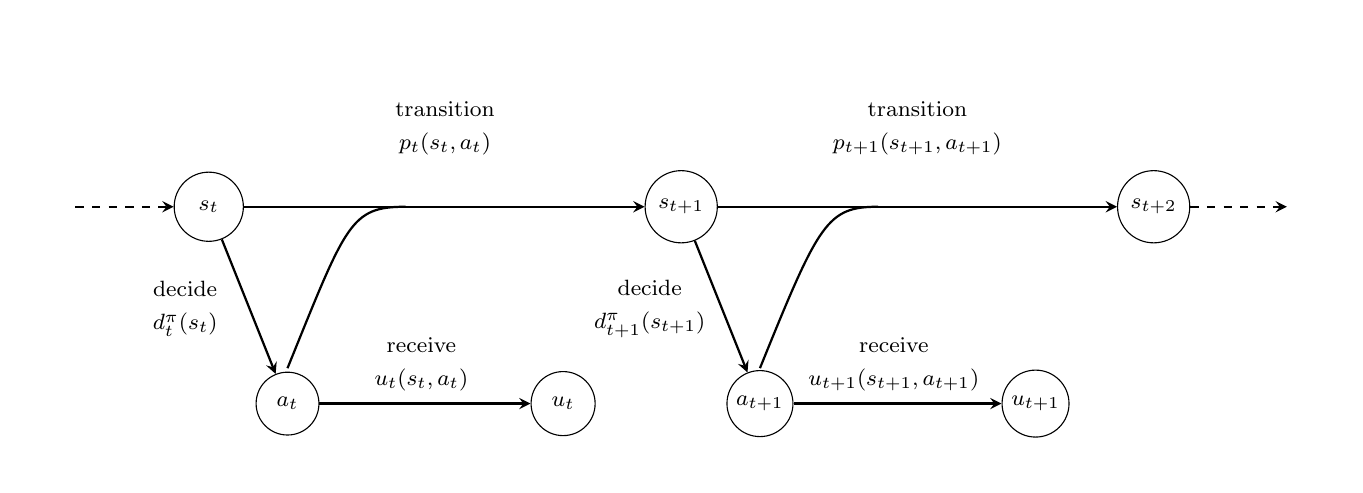
\begin{tikzpicture}[node distance=2cm]
%define styles
\tikzstyle{startstop} = [circle, rounded corners, minimum width=0.6cm, minimum height=0.3cm,text centered, draw=black]
[
->,
>=stealth',
auto,node distance=3cm,
thick,
main node/.style={circle, draw, font=\sffamily\Large\bfseries}
]
\tikzstyle{arrow} = [thick,->,>=stealth]]
\tikzstyle{darrow} = [dotted,->,>=stealth]]
%first and second column

\node (r0) [startstop, xshift = -3cm, draw = none] {};
\node (r999) [startstop, xshift = 13cm, draw = none] {};

\node (r1) [startstop, xshift = -1cm] {\footnotesize $~\,s_t\,~$};
\node (r2) [startstop, xshift = 5cm] {\footnotesize $s_{t+1}$};  %previously 4
\node (r3) [startstop, xshift = 11cm] {\footnotesize $s_{t+2}$}; %previously 8

\draw [arrow, dashed] (r0) -- node[anchor=south] {} (r1) ;
\draw [arrow] (r1) -- node[anchor=south] {} (r2) ;
\draw [arrow] (r2) -- node[anchor=south] {} (r3) ;
\draw [arrow, dashed] (r3) -- node[anchor=south] {} (r999) ;
t
\node (r4) [startstop, xshift = 0 cm, yshift = -2.5cm, inner sep = 0.08cm] {\footnotesize $~\,a_t\,~$ };
\node (r5) [startstop, xshift = 3.5
 cm, yshift = -2.5cm, inner sep = 0.08cm] {\footnotesize $~\,u_t\,~$ };
\node (r6) [startstop, xshift = 6 cm, yshift = -2.5cm, inner sep = 0.08cm] {\footnotesize $a_{t+1}$ };
\node (r7) [startstop, xshift = 9.5 cm, yshift = -2.5cm, inner sep = 0.08cm] {\footnotesize $u_{t+1}$ };

\draw [arrow] (r1) -- node[anchor=south] {} (r4) ;
\draw [arrow] (r2) -- node[anchor=south] {} (r6) ;

\draw[ thick](0,-2.05).. controls (0.75, -0.2) and (0.8,0)..(1.5, 0);
\draw [arrow] (r4) -- node[anchor=south] {} (r5) ;
\draw[ thick](6,-2.05).. controls (6.75, -0.2) and (6.85,0)..(7.5, 0);
\draw [arrow] (r6) -- node[anchor=south] {} (r7) ;


\node(r8)[startstop, xshift = - 1.3cm, yshift = -1.3cm, draw =none, align=center] {\footnotesize decide \\ \footnotesize $d_t^{\pi}(s_t)$ };
\node(r9)[startstop, xshift= 4.6cm, yshift = -1.3cm, draw =none, align = center] {\footnotesize decide \\ \footnotesize $d_{t+1}^{\pi}(s_{t+1})$ };
\node(r10)[startstop, yshift = 1cm, xshift = 2cm, draw =none, align=center ] {\footnotesize transition \\ \footnotesize $p_t(s_t, a_t)$};
\node(r11)[startstop, yshift = 1cm, xshift = 8cm, draw =none, align=center ] { \footnotesize transition \\ \footnotesize $p_{t+1}(s_{t+1}, a_{t+1})$};
%\node(r10)[startstop, yshift = 0.5cm, xshift = 1.7cm, draw =none, align=center ] {\footnotesize transition \\ \footnotesize $p(s_t, a_t)$};
%\node(r11)[startstop, yshift = 0.5cm, xshift = 8cm, draw =none, align=center ] {\footnotesize transition \\ \footnotesize $p(s_{t+1}, a_{t+1})$};
\node(r12)[startstop, yshift = -2cm, xshift = 1.7cm, draw =none, align=center ] {\footnotesize receive\\ \footnotesize $u_t(s_t, a_t)$};
\node(r13)[startstop, yshift = -2cm, xshift = 7.7cm, draw =none, align=center ] {\footnotesize receive\\ \footnotesize $u_{t+1}(s_{t+1}, a_{t+1})$};

\end{tikzpicture}
}
\end{frame}
%---------------------------------------------------------------------------------------------------
%---------------------------------------------------------------------------------------------------
\begin{frame}\frametitle{Individual's objective}\vspace{0.3cm}

\begin{multicols}{2}

\begin{align*}
\max_{\pi \in\Pi} \E_{s_1}^\pi\left[\sum^{T}_{t = 1}  \delta^{t - 1} u_t(s_t, a^\pi_t(s_t))\right]
\end{align*}

\columnbreak

\heading{Core economics}\vspace{0.3cm}
\begin{itemize}\setlength\itemsep{1em}
   \item Rational expectations
   \item Exponential discounting
   \item Time-separability
\end{itemize}

\end{multicols}

\end{frame}
%---------------------------------------------------------------------------------------------------
%---------------------------------------------------------------------------------------------------
\begin{frame}{Seminal paper}\vspace{0.65cm}
\fullcite{Keane.1997}.\vspace{0.5cm}

\begin{itemize}\setlength\itemsep{1em}
	\item The study follows individuals over their working life from young adulthood at age 16 to retirement at age 65 where the decision period $t = 16, \dots, 65$  is a school year.
	\item Individuals decide $a\in\mathcal{A}$ whether to work in a blue-collar or white-collar occupation ($a = 1, 2$), to serve in the military $(a = 3)$, to attend school $(a = 4)$, or to stay at home $(a = 5)$.
	\item Authors use the model to predict and understand the effects of numerous human capital policies.
\end{itemize}


\end{frame}
%---------------------------------------------------------------------------------------------------
%---------------------------------------------------------------------------------------------------
\begin{frame}{Decision tree}

\begin{figure}
  \scalebox{0.60}{% Decision tree

\tikzset{
	treenode/.style = {shape=rectangle, rounded corners, draw, align=center, bottom color=blue!20},
	root/.style     = {treenode, font=\small, draw=none},
	env/.style      = {treenode, font=\small, draw=none},
	dummy/.style    = {circle,draw}
}


\begin{tikzpicture}
[
	x=30pt,
	y=26pt,
	yscale=-1,
	xscale=1,
	baseline=-120pt,
	grow                    = right,
	edge from parent/.style = {draw, -latex},
	%every node/.style       = {font=\footnotesize, minimum width={width%("Magnetometer")
			%+2pt}},
			every node/.style       = {font=\footnotesize, minimum width={2cm}},
	sloped
]


% Zero  level: START
\node [root, top color = tabgrey, bottom color = tabgrey, color = white] (0) at (-10,0) {\textbf{Start}};


% First level: BLUE
\node [env, top color = tabblue, bottom color = tabblue, color = white, scale = 0.8] (1) at (-5,-4.2) {\textbf{Blue}};
\draw[->, thick] (0) edge node[left of = 0, rotate = 72.75, node distance = 0.3cm]{} (1);
% Second level: Blue, White, Military, School, Home
\node [env, top color = tabblue, bottom color = tabblue, color = white, scale = 0.55] (11) at (0,-5) {Blue};
\draw[->] (1) edge (11);
\node [env, top color = tabred, bottom color = tabred, color = white, scale = 0.55] (12) at (0,-4.6) {White};
\draw[->] (1) edge (12);
\node [env, top color = tabpurple, bottom color = tabpurple, color = white, scale = 0.55] (13) at (0,-4.2) {Military};
\draw[->] (1) edge (13);
\node [env, top color = taborange, bottom color = taborange, color = white, scale = 0.55] (14)  at (0,-3.8) {School};
\draw[->] (1) edge (14);
\node [env, top color = tabgreen, bottom color = tabgreen, color = white, scale = 0.55] (15)  at (0,-3.4) {Home};
\draw[->] (1) edge (15);
% Third level coordinates
\coordinate (a1) at (3,-5);
\draw [->, dashed, color = tabgrey] (11) to[right] node[auto] {} (a1);
\coordinate (a2) at (3,-4.6);
\draw [->, dashed, color = tabgrey] (12) to[right] node[auto] {} (a2);
\coordinate (a3) at (3,-4.2);
\draw [->, dashed, color = tabgrey] (13) to[right] node[auto] {} (a3);
\coordinate (a4) at (3,-3.8);
\draw [->, dashed, color = tabgrey] (14) to[right] node[auto] {} (a4);
\coordinate (a5) at (3,-3.4);
\draw [->, dashed, color = tabgrey] (15) to[right] node[auto] {} (a5);



%First level: WHITE
\node [env, top color = tabred, bottom color = tabred, color = white, scale = 0.8] (2) at (-5,-2.1) {\textbf{White}};
\draw[->, thick] (0) edge node[right of = 0, yshift = 0.35cm, rotate = 41.0, node distance = 0cm]{} (2);
% Second level: Blue, White, Military, School, Home
\node [env, top color = tabblue, bottom color = tabblue, color = white, scale = 0.55] (21) at (0,-2.9) {Blue};
\draw[->] (2) edge (21);
\node [env, top color = tabred, bottom color = tabred, color = white, scale = 0.55] (22) at (0,-2.5) {White};
\draw[->] (2) edge (22);
\node [env, top color = tabpurple, bottom color = tabpurple, color = white, scale = 0.55] (23) at (0,-2.1) {Military};
\draw[->] (2) edge (23);
\node [env, top color = taborange, bottom color = taborange, color = white, scale = 0.55] (24)  at (0,-1.7) {School};
\draw[->] (2) edge (24);
\node [env, top color = tabgreen, bottom color = tabgreen, color = white, scale = 0.55] (25)  at (0,-1.3) {Home};
\draw[->] (2) edge (25);
% Second level --> third level
\coordinate (e1) at (3,-2.9);
\draw [->, dashed, color = tabgrey] (21) to[right] node[auto] {} (e1);
\coordinate (e2) at (3,-2.5);
\draw [->, dashed, color = tabgrey] (22) to[right] node[auto] {} (e2);
\coordinate (e3) at (3,-2.1);
\draw [->, dashed, color = tabgrey] (23) to[right] node[auto] {} (e3);
\coordinate (e4) at (3,-1.7);
\draw [->, dashed, color = tabgrey] (24) to[right] node[auto] {} (e4);
\coordinate (e5) at (3,-1.3);
\draw [->, dashed, color = tabgrey] (25) to[right] node[auto] {} (e5);


% First Level: MILITARY
\node [env, top color = tabpurple, bottom color = tabpurple, color = white, scale = 0.8] (3) at (-5,0) {\textbf{Military}};
\draw[->, thick] (0) edge node[right of = 0, yshift = 0.25cm, node distance = 0.2cm]{} (3);
% Second level: Blue, White, Military, School, Home
\node [env, top color = tabblue, bottom color = tabblue, color = white, scale=0.55] (31) at (0,-0.8) {Blue};
\draw[->] (3) edge (31);
\node [env, top color = tabred, bottom color = tabred, color = white, scale = 0.55] (32) at (0,-0.4) {White};
\draw[->] (3) edge (32);
\node [env, top color = tabpurple, bottom color = tabpurple, color = white, scale = 0.55] (33) at (0,0.0) {Military};
\draw[->] (3) edge (33);
\node [env, top color = taborange, bottom color = taborange, color = white, scale = 0.55] (34)  at (0,0.4) {School};
\draw[->] (3) edge (34);
\node [env, top color = tabgreen, bottom color = tabgreen, color = white, scale = 0.55] (35)  at (0,0.8) {Home};
\draw[->] (3) edge (35);
% Second level --> third level
\coordinate (c1) at (3,-0.8);
\draw [->, dashed, color = tabgrey] (31) to[right] node[auto] {} (c1);
\coordinate (c2) at (3,-0.4);
\draw [->, dashed, color = tabgrey] (32) to[right] node[auto] {} (c2);
\coordinate (c3) at (3,0);
\draw [->, dashed, color = tabgrey] (33) to[right] node[auto] {} (c3);
\coordinate (c4) at (3,0.4);
\draw [->, dashed, color = tabgrey] (34) to[right] node[auto] {} (c4);
\coordinate (c5) at (3,0.8);
\draw [->, dashed, color = tabgrey] (35) to[right] node[auto] {} (c5);


% First Level: SCHOOL
\node [env, top color = taborange, bottom color = taborange, color = white, scale = 0.8] (4)  at (-5,2.1) {\textbf{School}};
\draw[->, thick] (0) edge node[right of = 0, yshift = 0.1cm, rotate = -38, node distance = 0.25cm]{} (4);
% Second level: Blue, White, Military, School, Home
\node [env, top color = tabblue, bottom color = tabblue, color = white, scale = 0.55] (41) at (0,1.3) {Blue};
\draw[->] (4) edge (41);
\node [env, top color = tabred, bottom color = tabred, color = white, scale = 0.55] (42) at (0,1.7) {White};
\draw[->] (4) edge (42);
\node [env, top color = tabpurple, bottom color = tabpurple, color = white, scale = 0.55] (43) at (0,2.1) {Military};
\draw[->] (4) edge (43);
\node [env, top color = taborange, bottom color = taborange, color = white, scale = 0.55] (44)  at (0,2.5) {School};
\draw[->] (4) edge (44);
\node [env, top color = tabgreen, bottom color = tabgreen, color = white, scale = 0.55] (45)  at (0,2.9) {Home};
\draw[->] (4) edge (45);
% Second level --> third level
\coordinate (b1) at (3,1.3);
\draw [->, dashed, color = tabgrey] (41) to[right] node[auto] {} (b1);
\coordinate (b2) at (3,1.7);
\draw [->, dashed, color = tabgrey] (42) to[right] node[auto] {} (b2);
\coordinate (b3) at (3,2.1);
\draw [->, dashed, color = tabgrey] (43) to[right] node[auto] {} (b3);
\coordinate (b4) at (3,2.5);
\draw [->, dashed, color = tabgrey] (44) to[right] node[auto] {} (b4);
\coordinate (b5) at (3,2.9);
\draw [->, dashed, color = tabgrey] (45) to[right] node[auto] {} (b5);


% First Level: HOME
\node [env, top color = tabgreen, bottom color = tabgreen, color = white, scale = 0.8] (5)  at (-5,4.2) {\textbf{Home}};
\draw[->, thick] (0) edge node[right of = 0, yshift=0.25cm, rotate = -72.75, node distance = 0.15cm]{} (5);
%\draw[->, thick] (0) edge (5);
% Second level: Blue, White, Military, School, Home
\node [env, top color = tabblue, bottom color = tabblue, color = white, scale = 0.55] (51)  at (0,3.4) {Blue};
\draw[->] (5) edge (51);
\node [env, top color = tabred, bottom color = tabred, color = white, scale = 0.55] (52)  at (0,3.8) {White};
\draw[->] (5) edge (52);
\node [env, top color = tabpurple, bottom color = tabpurple, color = white, scale = 0.55] (53) at (0,4.2) {Military};
\draw[->] (5) edge (53);
\node [env, top color = taborange, bottom color = taborange, color = white, scale = 0.55] (54) at (0,4.6) {School};
\draw[->] (5) edge (54);
\node [env, top color = tabgreen, bottom color = tabgreen, color = white, scale = 0.55] (55) at (0,5.0) {Home};
\draw[->] (5) edge (55);
% Second level --> third level
\coordinate (d1) at (3,3.4);
\draw [->, dashed, color = tabgrey] (51) to[right] node[auto] {} (d1);
\coordinate (d2) at (3,3.8);
\draw [->, dashed, color = tabgrey] (52) to[right] node[auto] {} (d2);
\coordinate (d3) at (3,4.2);
\draw [->, dashed, color = tabgrey] (53) to[right] node[auto] {} (d3);
\coordinate (d4) at (3,4.6);
\draw [->, dashed, color = tabgrey] (54) to[right] node[auto] {} (d4);
\coordinate (d5) at (3,5.0);
\draw [->, dashed, color = tabgrey] (55) to[right] node[auto] {} (d5);

\end{tikzpicture}

\vspace{1cm}
}
\end{figure}
\end{frame}

%---------------------------------------------------------------------------------------------------
%---------------------------------------------------------------------------------------------------
\begin{frame}\frametitle{Immediate utility}\vspace{0.3cm}

  \begin{multicols}{2}

  \begin{align*}
  u_t(s_t) =
  \begin{cases}
      \,\zeta_a(s_t)  + w_a(s_t)   & \text{if}\, a \in \{1, 2, 3\}  \\[0.2cm]
      \,\zeta_a(s_t)                 &  \text{if}\, a \in \{4, 5\}
  \end{cases}
  \end{align*}

  \columnbreak


  \heading{Informed by reduced-form evidence}\vspace{0.3cm}
  \begin{itemize}\setlength\itemsep{1em}
     \item Mincer equation
     \item Diploma effects
     \item Skill depreciation
     \item Mobility and search costs
     \item Monetary and psychic cost of schooling
  \end{itemize}

\end{multicols}

\end{frame}
%---------------------------------------------------------------------------------------------------
%---------------------------------------------------------------------------------------------------
\begin{frame}{Transitions}\vspace{0.25cm}

\begin{itemize}\setlength\itemsep{1em}
  \item Work experience $\bm{k}_t$  and years of completed schooling $h_t$ evolve deterministically.
  \begin{align*}
  k_{a,t+1} = k_{a,t} + \ind[a_t = a]  &\qquad \text{if}\, a \in \{1, 2, 3\} \\
  h_{t + 1\phantom{,a}} = h_{t\phantom{,a}} +   \ind[a_t = 4]  &\qquad
  \end{align*}


  \item Productivity shocks $\bm{\epsilon}_t$ are uncorrelated across time and follow a multivariate normal distribution with mean $\bm{0}$ and covariance matrix $\bm{\Sigma}$.

  \item Given the structure of the utility functions and the distribution of the shocks, the state at time $t$ is $s_t = \{\bm{k}_t, h_t, t, a_{t -1}, \bm{e},\bm{\epsilon}_t\}$.
\end{itemize}

\end{frame}
%---------------------------------------------------------------------------------------------------
%---------------------------------------------------------------------------------------------------
\begin{frame}{Utility of schooling}\vspace{0.25cm}

\begin{align*}
		\zeta_4(s_t)   = & \underbrace{e_{j,4}}_{\text{type}} + \underbrace{\beta_{tc_1} \cdot \ind[h_t \geq 12] + \beta_{tc_2} \cdot \ind[h_t \geq 16]}_{\color{red}\text{tuition costs}}  + \underbrace{\gamma_{4,4} \cdot t + \gamma_{4,5} \cdot \ind[t < 18]}_{\text{time trend}}  \\[15pt]
	    							  & + \underbrace{\beta_{rc_1} \cdot \ind[a_{t-1} \neq 4, h_t < 12]   + \beta_{rc_2} \cdot \ind[a_{t-1} \neq 4, h_t \geq 12]}_{\text{re-enrollment cost}}  + \hdots + \epsilon_{4,t}
\end{align*}


\end{frame}\addtocounter{framenumber}{-1}
%---------------------------------------------------------------------------------------------------
%---------------------------------------------------------------------------------------------------
\begin{frame}{Utility of schooling}\vspace{0.25cm}

\begin{align*}
		\zeta_4(s_t)   = & \underbrace{e_{j,4}}_{\color{red}\text{type}} + \underbrace{\beta_{tc_1} \cdot \ind[h_t \geq 12] + \beta_{tc_2} \cdot \ind[h_t \geq 16]}_{\text{tuition costs}}  + \underbrace{\gamma_{4,4} \cdot t + \gamma_{4,5} \cdot \ind[t < 18]}_{\text{time trend}}  \\[15pt]
	    							  & + \underbrace{\beta_{rc_1} \cdot \ind[a_{t-1} \neq 4, h_t < 12]   + \beta_{rc_2} \cdot \ind[a_{t-1} \neq 4, h_t \geq 12]}_{\text{re-enrollment cost}}  + \hdots + \epsilon_{4,t}
\end{align*}


\end{frame}
%---------------------------------------------------------------------------------------------------
%---------------------------------------------------------------------------------------------------
\begin{frame}{National Longitudinal Survey of Youth 1979}\vspace{0.25cm}

	\begin{itemize}\setlength\itemsep{1em}
	\item 1,373 individuals starting at age 16
	\item Life cycle histories\medskip
	\begin{itemize}\setlength\itemsep{1em}
		\item School attendance
		\item Occupation-specific work status
		\item Wage\medskip
	\end{itemize}
	\item Likelihood-based estimation
\end{itemize}

\end{frame}
%---------------------------------------------------------------------------------------------------
%---------------------------------------------------------------------------------------------------
\begin{frame}{Data descriptives}
  \begin{figure}[h!]\centering
  \subfloat[Choices]{\scalebox{0.225}{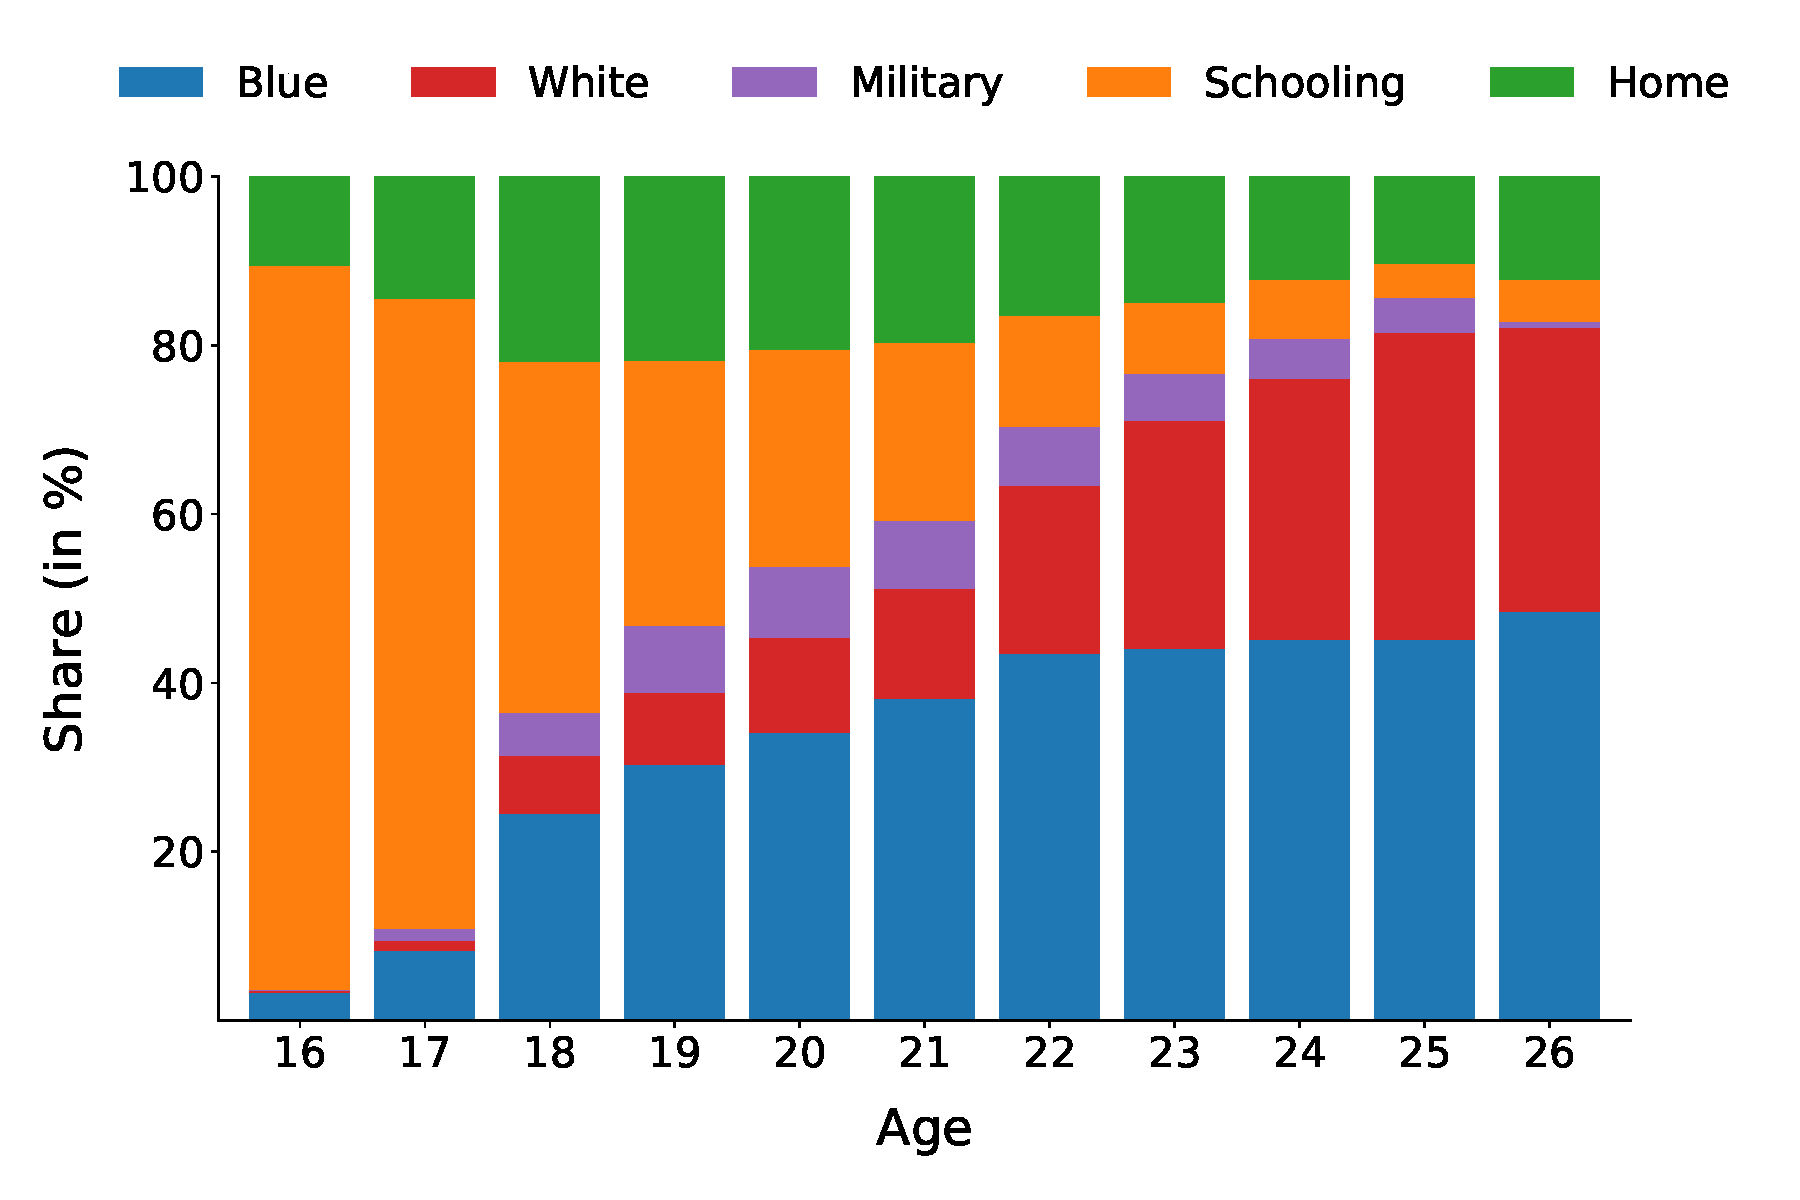
\includegraphics{fig-observed-data-choices}}}\hspace{0.5cm}
  \subfloat[Wages]{\scalebox{0.225}{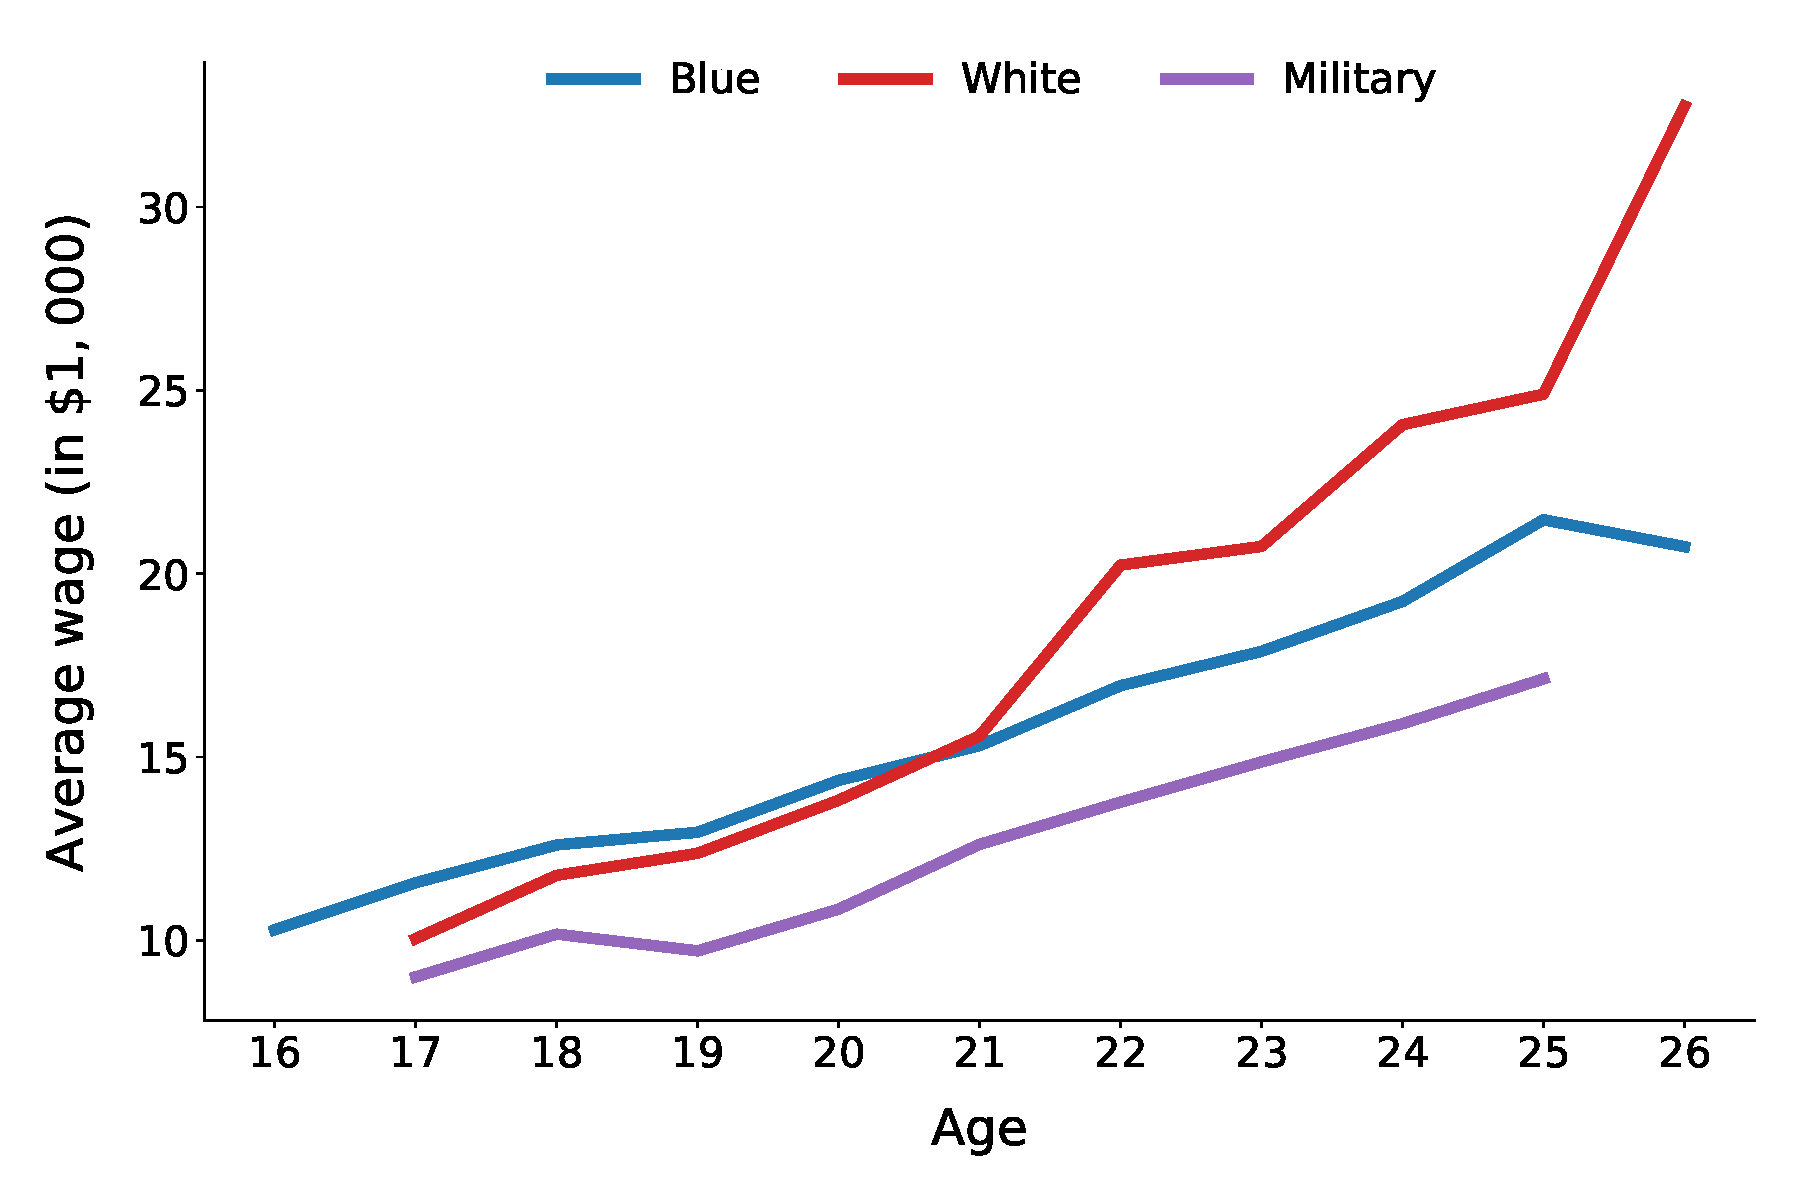
\includegraphics{fig-observed-wage-mean}}}
  \end{figure}
\end{frame}
%---------------------------------------------------------------------------------------------------
%---------------------------------------------------------------------------------------------------
\begin{frame}{Determining the confidence set}\vspace{0.25cm}

We implement the Confidence Set bootstrap \citep{Rao.1973,Woutersen.2019}.\vspace{0.3cm}

\pause
\begin{enumerate}\setlength\itemsep{1em}
  \item We draw a large sample of $\hat{\btheta}_{m}$ from the asymptotic distribution of our estimates.
  \item We keep draws that are elements of the estimated confidence set $\hat{\bTheta}(\alpha)$.
  \item We compute $\hat{y}_{g,m}$ for all remaining draws.
  \item We calculate the uncertainty set $\U_{y_g}(\alpha)$ based on the lowest and highest value of $\hat{y}_{g,m}$.
\end{enumerate}\vspace{1.0cm}

\hyperlink{fig:algorithmic-description}{\beamerbutton{Algorithmic description}}
\label{determine-confidence-set}
\end{frame}
%---------------------------------------------------------------------------------------------------
%---------------------------------------------------------------------------------------------------
